% Define Document Class to be used and options %
\documentclass[12pt,a4paper]{article}
%\renewcommand{\rmdefault}{ma1}
%-------------------------------------C:\Program Files\MiKTeX 2.5\miktex----------------------------------%
% Preamble %

% Define Packages To be used and options %
% here you define all the packages you wish to use in your paper, the ones shown are not all necessary,
% but all have purpose and can be very useful, so leave these as default and add packages as necassary
\usepackage[dvipdfm]{graphicx}
\usepackage{xcolor}
\usepackage{amsmath}
\usepackage{amsthm}
\usepackage{multirow}
\usepackage{url}
\usepackage{longtable}
\usepackage{amsfonts}
\usepackage{amssymb}
\usepackage[numbers]{natbib}
\usepackage{hyperref}
\usepackage{hhline}


%------------------------------------------%

% user defined commands in order to geC:\Program Files\MiKTeX 2.5\miktexnerate new commands, macros, and redefine default commands %
\include{usersetcommands}

%-------------------------------------------------------------------------------------------------------%

% Begin Main Part of Document %

%\renewcommand{\rmdefault}{cmss}
%\renewcommand{\rmdefault}{ma1}
%\renewcommand{\sfdefault}{ma1}
%\renewcommand{\rmdefault}{mns}
%\renewcommand{\rmdefault}{ma1}
%\renewcommand{\rmdefault}{mns}
%\renewcommand{\rmdefault}{ma1}
%\renewcommand{\rmdefault}{cmss}
%\renewcommand{\rmdefault}{ma1}
%\renewcommand{\sfdefault}{cmss}
%\renewcommand{\rmdefault}{@calibri}
%\renewcommand{\rmdefault}{@hatten}
%\renewcommand{\rmdefault}{@lsans}
\begin{document}

%\bibliographystyle{plain}
%\bibliographystyle{ufinit}
%\bibliographystyle{abbrvnat}
%\bibliographystyle{plainnat}
%\bibliographystyle{unsrtnat}
%\bibliographystyle{Chicago_Web}
%\bibliographystyle{apa-good}
%\bibliographystyle{uf_econ}
%\bibliographystyle{Science_Web}
%\bibliographystyle{unsrturl_uf}
%\bibliographystyle{abbrvurl_uf}
%\bibliographystyle{alphaurl_uf}
%\bibliographystyle{ecology_web}
\bibliographystyle{mla-good}
%\bibliographystyle{mla_web}
%\bibliographystyle{plainurl_uf}
%-----------------------------------------------------------------------%

%------------------------------------------%

%\dedication{\input{dedication}}

%------------------------------------------%

%\include{acknowledgements} %

%------------------------------------------%

%\include{abstract} %

%-----------------------------------------------------------------------%

% This section encompasses the main body of the paper from all the content through to the biographical sketch

% Chapters to be included (more can be added by creating a new chapter#.tex %
% file and then implementing the /inlcude{chapter#.tex} command as seen below %

%
%
\documentclass[10pt,a4paper]{article}
%\usepackage[latin1]{inputenc}
\usepackage{amsmath}
%\usepackage{amsfonts}
\usepackage{amssymb}
\usepackage{graphicx}
\usepackage{hyperref}
%\usepackage{vmargin}



%%%%%%%%%%%%%%%%%%%%%%%%%%%%%%
\title{The Advanced LIGO Input Mode Cleaner}
\author{Chris Mueller}
%\ligodraft
%%%%%%%%%%%%%%%%%%%%%%%%%%%%%%%%%%%%%%%%%%%%%%%%%%%%%%%%%%%%%%%%%%%%%
\begin{document}


%=================================================================================================
\section{Introduction}

A worldwide effort to directly detect gravitational radiation with large scale laser interferometers 
has been underway for the past several decades.  
In the United States the Laser Interferometer Gravitational-Wave Observatories (LIGO) have been operating
since the early 2000's.  
During this time of operation a significant amount of effort was invested by the LIGO Scientific Collaboration 
to research, design, and build upgrades to the initial LIGO interferometers.  
As of 2011 the initial LIGO detectors were decommissioned and installation of these upgrades began.  
As installation has progressed the integration and commissioning phase has begun for many of the 
upgraded subsystems at the LIGO observatories.  

One of the subsystems undergoing a significant upgrade for the Advanced LIGO era is 
the input optics.  
It is the task of the input optics to clean and stabilize the laser beam from the 
Pre-Stabilized Laser (PSL) before injection into the main interferometer.  
The upgraded sensitivity of the Advanced LIGO interferometers places stringent requirements on 
the stability of the input light and therefore on the input optics.  
In particular, the input optics must supply multiple low amplitude and phase noise RF sidebands.  
They must provide a frequency reference stable enough to not spoil the interferometer's 
gravitational wave sensitivity.  
They must provide mode matching and beam pointing actuation into the interferometer.  
Finally, they must provide isolation between the interferometer's reflected light and the 
input optics chain.  

The next section of this paper, section II, will present the design requirements for the input optics and 
briefly explain how these requirements were derived.  
It will also describe some of the other Advanced LIGO subsystems in only as much detail as 
is necessary for an understanding of the input optics.  
Sections III and IV will give an overview description of the out-of-vacuum and in-vacuum 
components respectively.  
Section V will discuss the input mode cleaner which is at the heart of the input optics, 
both in location and form.  
Section VI will describe the Faraday Isolator whose design is highly customized for high power 
operation.  
Finally, sections VII and IIX will close with a description of the overall power throughput of the 
input optics chain and some conclusions.  

%==================================================================================================
\section{Design Requirements}

The design requirements for the input optics subsystem derive from the designed sensitivity of the 
interferometer.  
Figure \ref{fig:aLIGODesignSensitivity} shows the design sensitivity of the Advanced LIGO interferometers 
together with the measured sensitivity of one of the Initial LIGO interferometers during the sixth 
science run.  
The Advanced LIGO interferometers are designed to be limited by seismic noise below $\sim$10 Hz, 
radiation pressure noise in the 10-50 Hz range, coating thermal noise between 50 Hz and 200 Hz, 
and photon shot noise above 200 Hz.  
The mantra for setting design requirements for the interferometer subsystems is therefore to keep 
the 'technical noise sources' below this limit.  
In fact the subsystem requirements were set by demanding that the technical noise sources be a factor of 
10 below the design sensitivity\cite{ligoT070236}.  

\begin{figure}
	\centering
	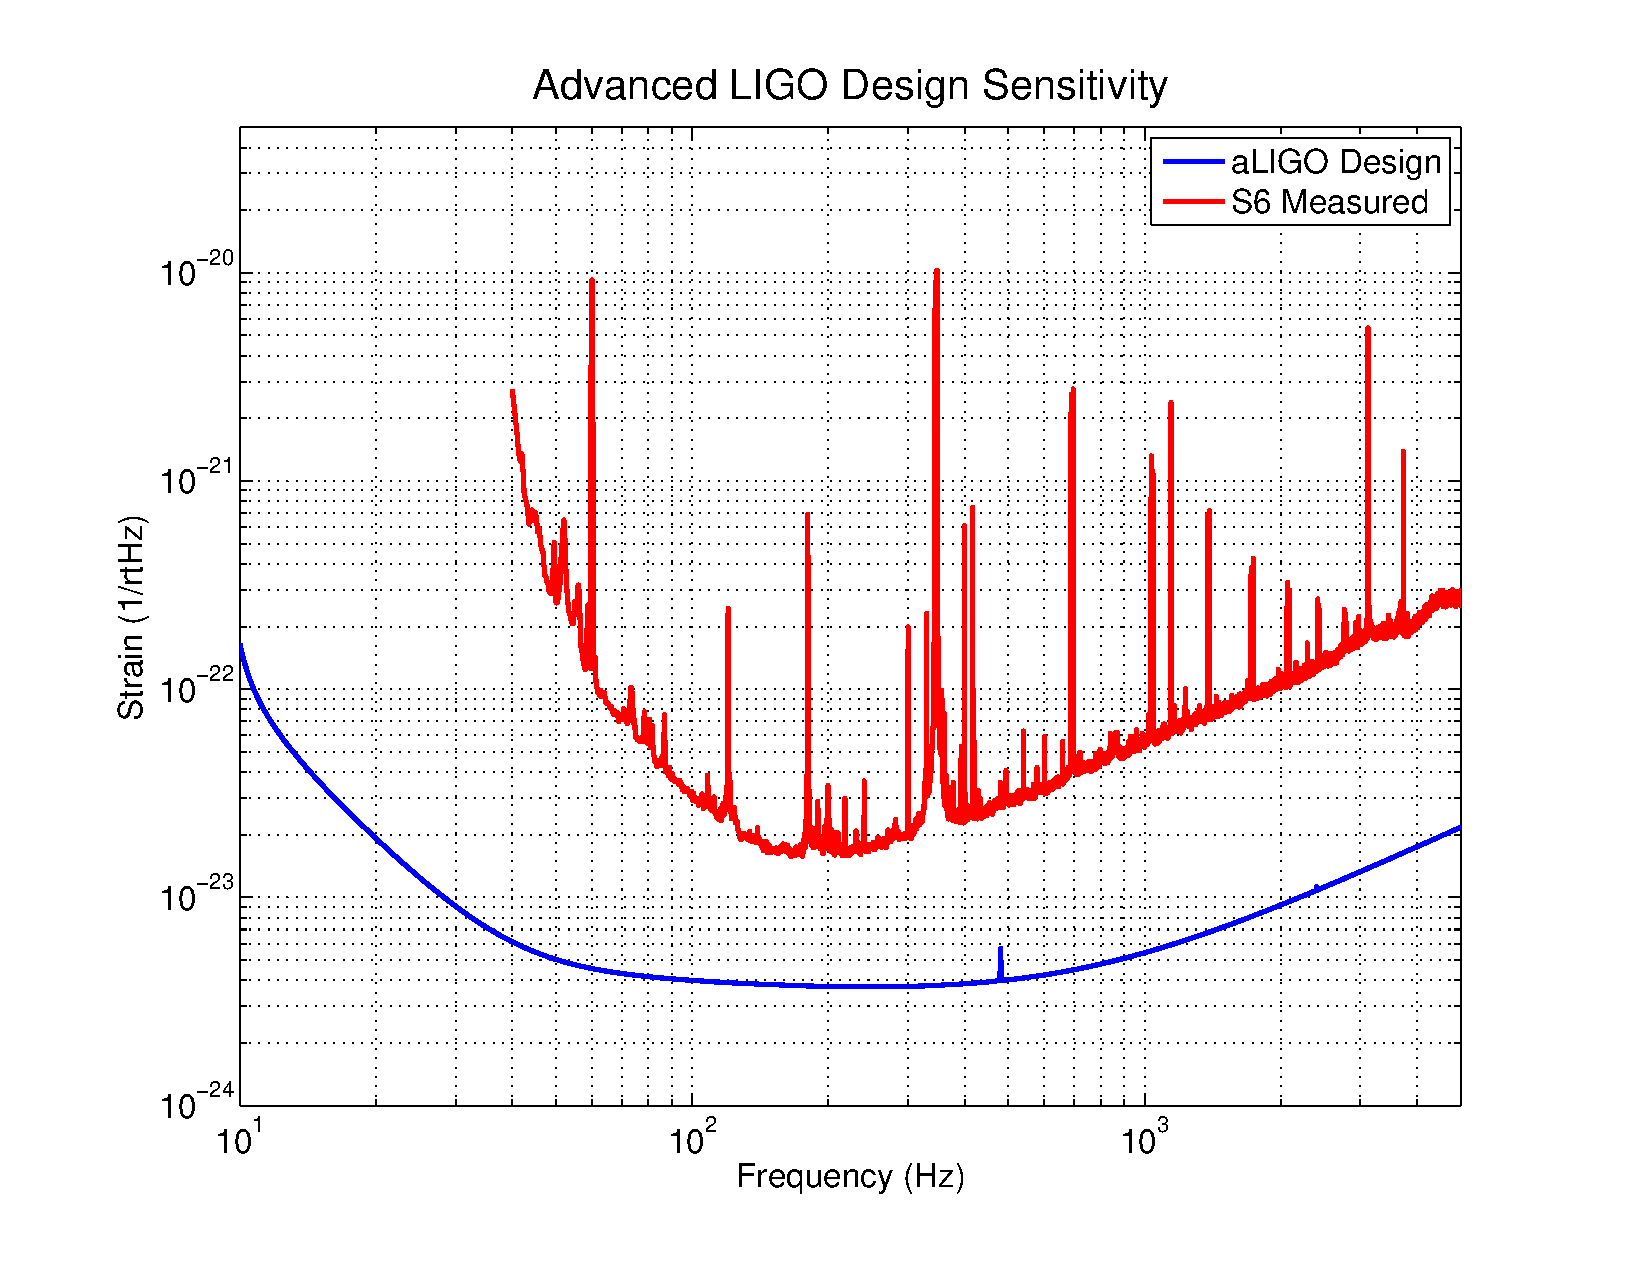
\includegraphics[width = 0.8\textwidth,trim=2cm 1cm 2cm 1cm]{aLIGO_Design_Sensitivity.pdf}
	\caption{The Advanced LIGO design sensitivity\cite{ligoT0900288} is shown together with the measured 
		sensitivity from the LIGO Hanford Observatory during the sixth LIGO science run\cite{ligoT1100388}.  
		The design sensitivity includes the fundamental limiting noise sources (quantum, thermal, and seismic) 
		which set the requirements for the interferometer subsystems such as the input optics.}
	\label{fig:aLIGODesignSensitivity}
\end{figure}

%--------------------------------------------------------------------------------------------------
\subsection{Frequency Noise at the Interferometer Input}

A perfect Michelson interferometer is completely insensitive to frequency noise; a fact which 
is a large motivator in choosing the Michelson topology for gravitational wave interferometers.  
However any asymmetry between the two arms of the Michelson interferometer will couple frequency 
fluctuations to the output.  
The asymmetries between the two arms depend on many parameters such as: the imbalance between the reflectivity 
and transmissivity of the beam splitter, the reflectivity imbalance of the arm cavity input mirrors, 
different amounts of losses in the two arm cavities, and the static distance asymmetry between the 
beam splitter and the two arm cavities (known as the Schnupp asymmetry).  

Using experience from Initial LIGO and a reasonable estimate of the Advanced LIGO parameters, 
the Interferometer Sensing and Control (ISC) group put together a detailed numerical simulation 
of the full Advanced LIGO interferometer \cite{ligoT070236}.  
With this simulation they derive the frequency noise requirement at the input to the interferometer 
to be roughly the curve labeled 'Frequency Noise Requirements at Interferometer Input' 
in figure \ref{fig:FreqReqs}.
The frequency noise stabilization for the interferometer is not solely the job of the input optics; 
the final stabilization reference is the average length of the two arms.  
Figure \ref{fig:FreqReqs} also shows the frequency noise requirements after suppression by the common 
arm length feedback servo.  
Also shown are the expected length noise of the input mode cleaner as well as the expected frequency 
noise out of the pre-stabilized laser.  

\begin{figure}
	\centering
	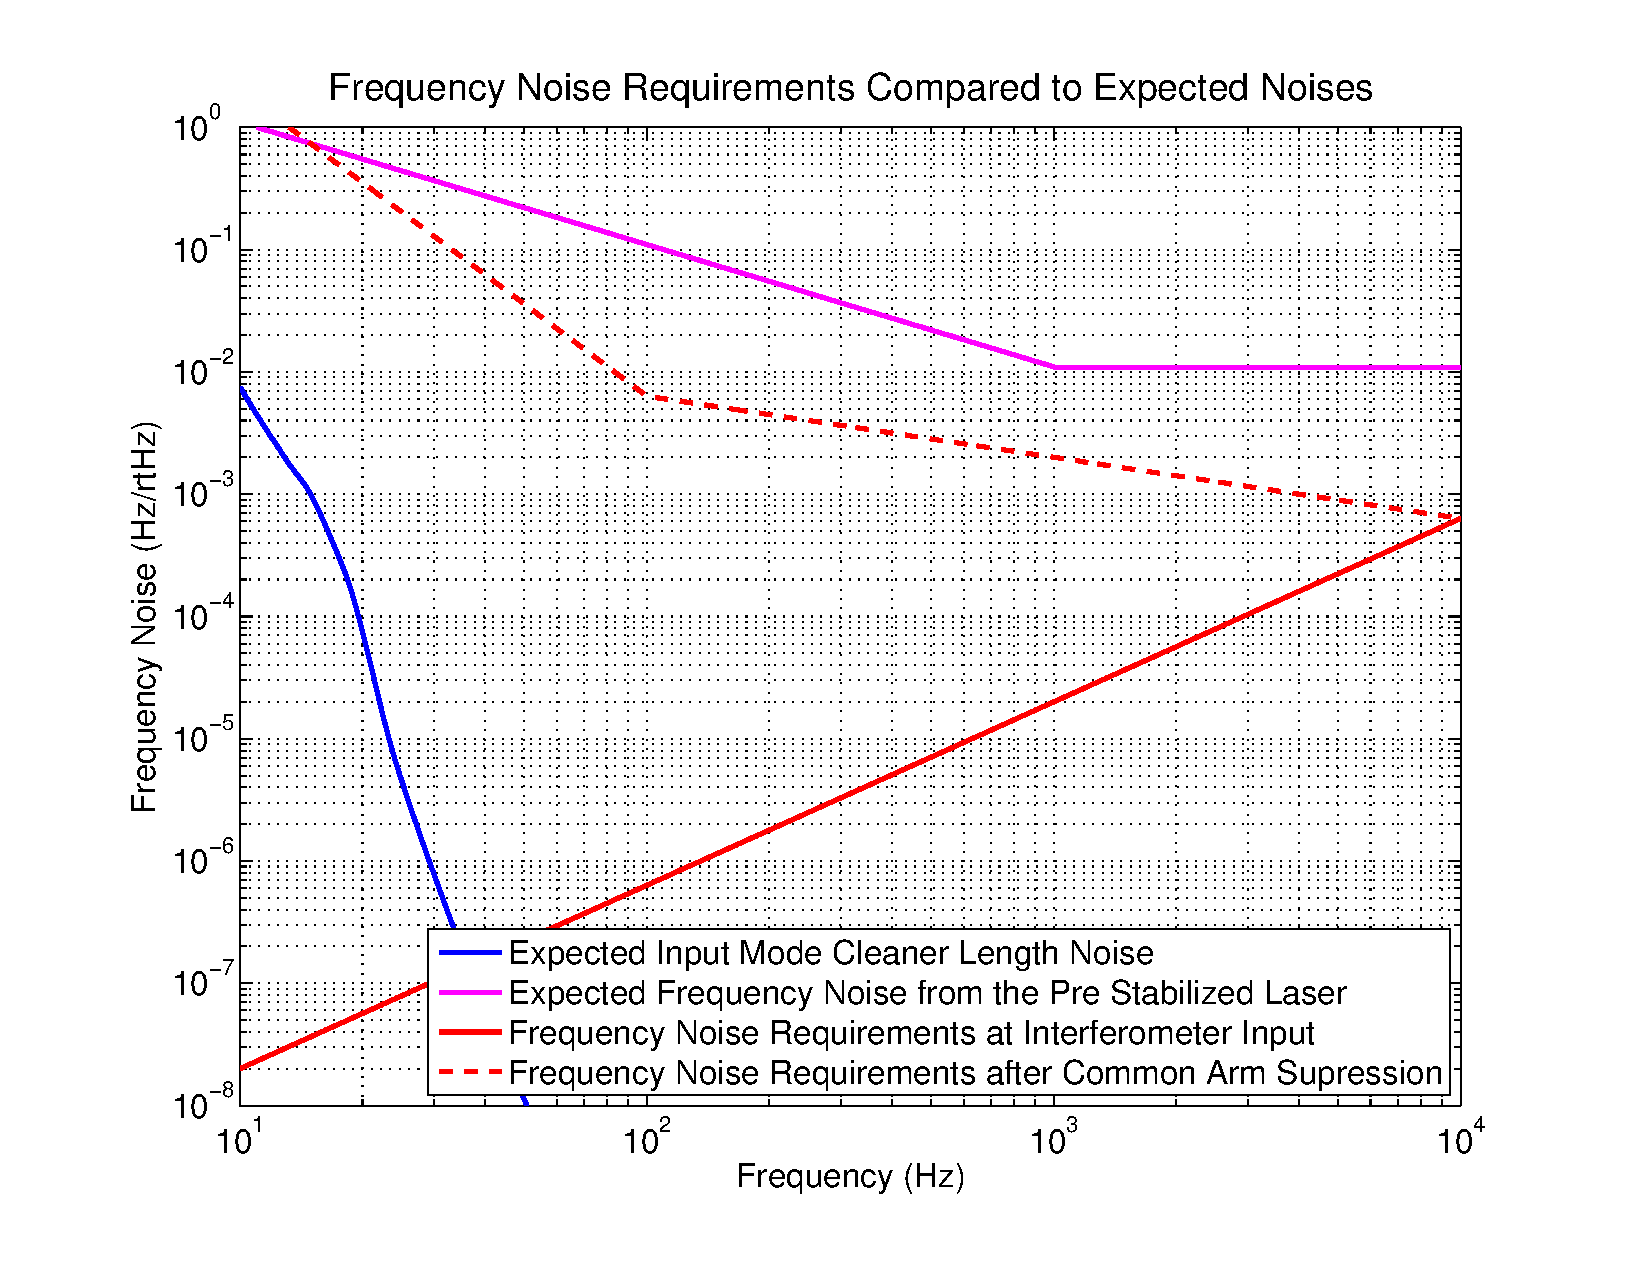
\includegraphics[width = 0.8\textwidth,trim=2cm 1cm 2cm 1cm]{Freq_Noise_Reqs.pdf}
	\caption{The rough frequency noise requirements at the input to the interferometer are shown both 
		with and without the common arm loop suppression.  
		Also shown are the expected length noise of the input mode cleaner and the expected frequency 
		noise out of the pre-stabilized laser (PSL).  
		Ostensibly the job of the input optics is to suppress the frequency noise out of the PSL to 
		the requirements level after the common arm gain is taken into account.  
		In reality acoustic effects in the injection optics between the PSL and the in-vacuum input 
		optics will require a higher level of suppression.}
	\label{fig:FreqReqs}
\end{figure}		

The job of the input optics is therefore to stabilize the laser frequency by roughly a factor of 20 
between 10 Hz and 10 kHz.  
In reality the frequency noise suppression necessary for the input optics is higher because 
acoustic effects in the injection chain will add frequency noise before the light is injected 
to the isolated in-vacuum optics.  


%--------------------------------------------------------------------------------------------------
\subsection{Beam Alignment Noise at the Interferometer Input}
As with frequency noise, a perfect Michelson interferometer is first order insensitive to pointing 
noise.  
There are two types of imperfections which couple pointing noise to the gravitational wave 
readout channel.  
The first considered in \cite{ligoT020022} is caused by residual misalignments of the core interferometer 
optics causing the misaligned beam to rejoin with the main interferometer mode and show up 
in the gravitational wave channel.  
The second coupling is caused by the beam spot motion on the core interferometer optics 
causing the residual angular motion of the optics to couple to the gravitational wave channel.
This effect is considered in \cite{ligoG1300442}.  
These two effects lead to similar noise requirements at the input to the interferometer which 
a beam stability of $4\cdot10^{-10}\ \frac{rad}{\sqrt{Hz}}$ at 100 Hz and above and decreasing 
(getting less stringent) as $f^2$ below 100 Hz.


%--------------------------------------------------------------------------------------------------
\subsection{RF Sidebands}
Sensing and controlling most of the seven degrees of freedom of the interferometer are done by some 
variant of the Pound Drever Hall technique \cite{PDH}.  
This technique uses optical heterodyne detection to sense the phase of the returning light from 
an optical cavity by sensing the phase modulation to amplitude modulation conversion which occurs 
when the cavity is slightly off resonance.  
It depends on having low noise radio frequency sidebands to generate detectable beat notes 
with the carrier light.
It is part of the responsibility of the input optics to add these RF sidebands to the laser beam 
before delivering it to the interferometer.  

In particular the input optics are responsible for adding three RF sidebands, one for controlling 
length of the input mode cleaner and two for controlling the other degrees of freedom of the 
interferometer.  
The phase modulator must be able to produce phase modulation depths up to 0.8, and must 
maintain a residual amplitude modulation level below $1\cdot10^{-4}$ $\frac{AM}{PM}$ ratio.  


%--------------------------------------------------------------------------------------------------
\subsection{In-Vacuum Optical Isolation}
The input optics is also required to provide isolation from the light reflected off of the 
interferometer.  
This is necessary to avoid inadvertently forming an optical cavity between the components 
of the input optics and the rest of the interferometer, 
an effect usually referred to as parasitic interferometry.  
Based on experience with parasitic interferometers in initial LIGO and power scaling arguments 
the isolation requirement level was set at 30 dB\cite{ligoT020020}.  


%--------------------------------------------------------------------------------------------------
\subsection{Throughput and Availability}
The final requirements on the input optics are placed on the amount of light which is delivered 
to the interferometer and the amount of time which the input mode cleaner is available.  
In order to deliver the 125 W of laser power required for full power operation the input optics 
must achieve 75\% throughput at all power levels including static and thermal mode matching losses.  
Additionally, in order not to spoil the detection availability of the interferometer 
it is required that the input mode cleaner re-lock time be less than 20 seconds.  

















\begin{thebibliography}{9}
	\bibitem{ligoT0900288} 
		LIGO-T0900288
	\bibitem{ligoT1100388}
		LIGO-T1100388	
	\bibitem{ligoT070236}
	  LIGO-T070236.  Interferometer Sensing and Control Design Requirements.
	\bibitem{ranasthesis}
		Rana's Thesis.  
	\bibitem{ligoT020022}
		LIGO-T020022. Guido's pointing noise doc.
	\bibitem{ligoG1300442}
		LIGO-G1300442. Lisa's pointing noise dcc. Maybe this doesn't need to be cited.  
	\bibitem{PDH}
		Drever Hall.  Laser Phase and Frequency Stabilization Using an Optical Resonator.		
	\bibitem{ligoT020020}
		LIGO-T020020. Input optics design requirements.	
\end{thebibliography}


\end{document}

\include{Design_Overview}
%
%
\documentclass[10pt,a4paper]{article}
%\usepackage[latin1]{inputenc}
\usepackage{amsmath}
%\usepackage{amsfonts}
\usepackage{amssymb}
\usepackage{graphicx}
\usepackage{hyperref}
%\usepackage{vmargin}



%%%%%%%%%%%%%%%%%%%%%%%%%%%%%%
\title{The Advanced LIGO Input Mode Cleaner}
\author{Chris Mueller}
%\ligodraft
%%%%%%%%%%%%%%%%%%%%%%%%%%%%%%%%%%%%%%%%%%%%%%%%%%%%%%%%%%%%%%%%%%%%%
\begin{document}

%%%%%%%%%%%%%%%%%%%%%%%%%%%%%%%%%%%%%%%%%%%%%%%%%%%%%%%%%%%%%%%%
\begin{large}
\begin{center}
\begin{LARGE}
\textbf{The Advanced LIGO Input Mode Cleaner}\\
\end{LARGE}
\vspace{0.50in}
\textbf{Chris Mueller} \\
Dept. of Physics, University of Florida\\
\today
\end{center}
\end{large}
\vspace{1pc}
\tableofcontents
\pagebreak[4]

%==================================================================================================
\section{Input Mode Cleaner}

The input mode cleaner is the heart of the input optics, serving simultaneously as a spatial filter, 
polarization filter, frequency reference, and pointing reference.  
It is an in-vacuum, suspended, three mirror cavity with the mirrors hanging from the LIGO small triple 
suspensions \textbf{citation}.  
It has a free spectral range of 9.099 MHz and a finesse of 515.  
The beam is injected along one of the long arms and extracted along the other (see \ref{fig:ioAll}).  
The reflected beam is outfitted with an RF photodiode for Pound-Drever-Hall length sensing \textbf{citation} 
and two wavefront sensors for angular control.  
In addition, a pickoff of the intra-cavity light is extracted behind the curved mirror, MC2, and sent to a 
quadrant photodiode for additional angular information.  

\begin{figure}
	\centering
	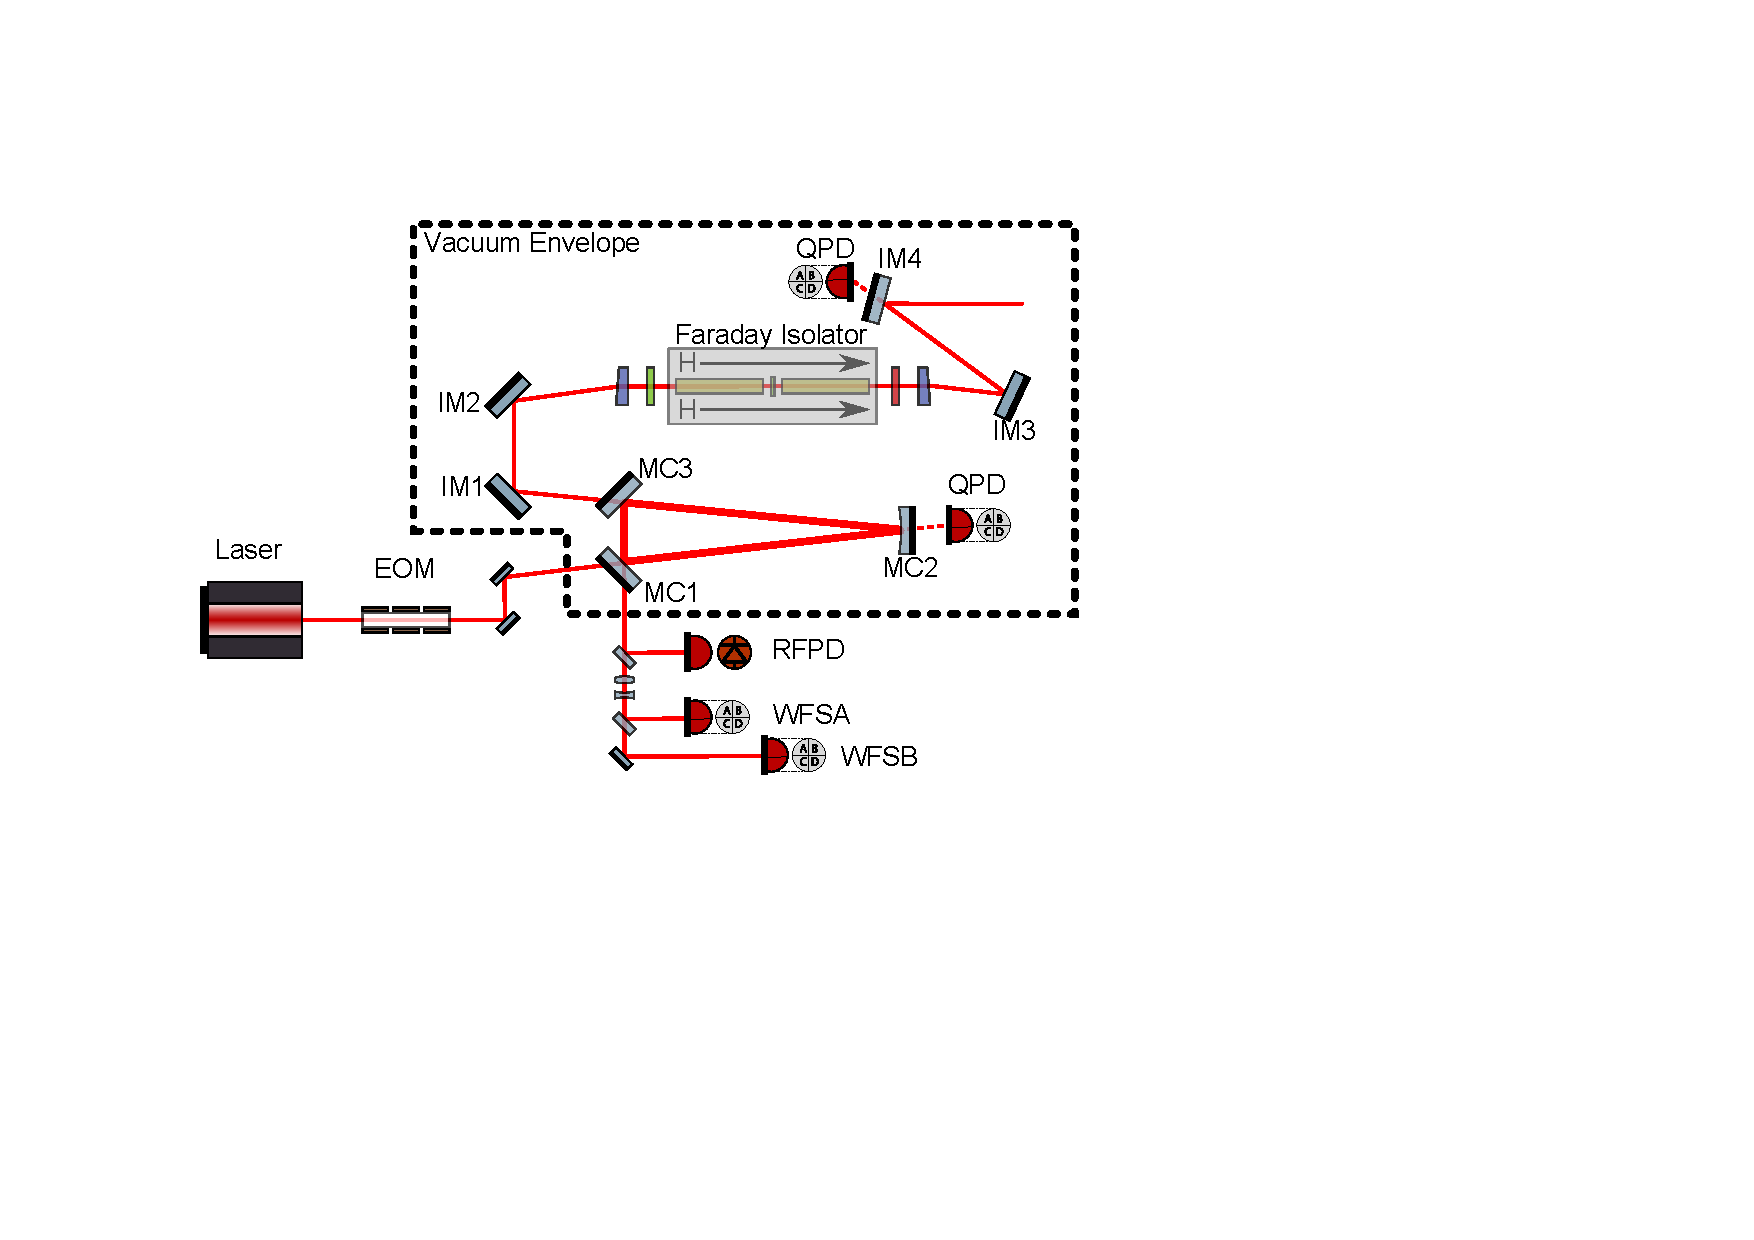
\includegraphics[width=0.9\textwidth, trim=3.5cm 7.5cm 11cm 3.5cm]{IO_Drawing.pdf}
	\caption{A schematic layout of the input optics is shown.  
		The input mode cleaner is represented by the three mirrors MC1, MC2, and MC3.  
		It is an in vacuum triply suspended triangular cavity used as a frequency 
		and pointing reference.  It also passively filters the spatial structure 
		and polarization of the incoming beam.}
	\label{fig:ioAll}
\end{figure}		

%--------------------------------------------------------------------------------------------------
\subsection{Power Budget}

%--------------------------------------------------------------------------------------------------
\subsection{Length Control}
Defining the reflectivity of MC1 and MC3 to be $r$ and assuming the cavity is lossless such that 
$t^2 = 1-r^2$ we can express the complex reflectivity of the cavity as 
\begin{equation}
	r_{IMC} = \frac{r(1+e^{-ik\ell})}{1+r^2e^{-ik\ell}},
\end{equation}
where $k$ is the spatial frequency of the light and $\ell$ is the round trip length of the cavity.  
Notice that this expression is identical to that of a 2 mirror impedance matched cavity except 
for the opposite sign in the denominator due to an odd number of mirrors.  

The most important aspect of this expression for our purposes is that the reflection coefficient 
undergoes a very rapid phase change from $-\pi/2$ on one side of the resonance to $\pi/2$ 
on the other side of the resonance, analogously to mechanical oscillators.  
This phase change can be detected by measuring the beat note between the light passing 
through resonance and a pair of RF sidebands.  
This technique is known as the Pound-Drever-Hall technique\cite{EricBlack}\cite{DreverHall} 
and allows for a very precise comparison between the length of the cavity and the frequency 
of the carrier light.  

As discussed in the requirements section \textbf{reference earlier section} one of the primary 
goals of the input optics is to quiet the laser frequency by at least an order of magnitude 
between 10 Hz and 10 kHz\textbf{reference earlier plot}.  
It is important however that the input optics not impress the length noise of the input mode 
cleaner at low frequencies where the laser frequency is much quieter.  
For this reason 

\begin{figure}
	\centering
	\includegraphics[width=0.8\textwidth,trim = 2.5cm 2cm 2.5cm 1.5cm]{Open_Loop_Tfs.pdf}
	\caption{A model of the open loop transfer functions of the various actuators in the 
		input mode cleaner length/frequency control servo.  
		The triple pendulum suspension of the MC2 mirror is used in a hierarchical scheme to 
		control the length of the cavity at low frequency using the laser frequency as a reference.  
		At higher frequencies the length of the input mode cleaner is more stable and the feedback 
		signal is instead used to stabilize the laser frequency.}
	\label{fig:ControlLoops}
\end{figure}		


%--------------------------------------------------------------------------------------------------
\subsection{Angular Control}

%--------------------------------------------------------------------------------------------------
\subsection{Cavity Pole}
If we define the reflectivity of MC1 and MC3 as $r$ and consider MC2 to be completely reflective, 
then we can express the transmissivity of the IMC as
\begin{equation}
	t_{IMC}=\frac{-t^2e^{-ik(\ell-\ell_3)}}{1+r^2e^{-ik\ell}}.
\end{equation}
Here $t$ is the transmissivity of MC1 and MC3, $\ell$ is the total round trip length, 
$\ell_3$ is the distance from MC1 to MC3, and $k=\tfrac{2\pi f}{c}$ is the spatial frequency 
of the light.  
The cavity is on resonance when $k\ell$ is a equal to $2n\pi+1$ for any $n\in\mathbb{Z}$.  
Notice that transmissivity of the cavity looks identical to that of an impedance matched 
two mirror cavity except for the static phase shift $e^{ik\ell_3}$.  

If we consider the transmissivity of frequencies very near the resonance frequency, 
then we are justified in Taylor expanding the exponential on the bottom to first order 
and the one on the top to 0th order.
Doing so gives an expression which looks like a single pole transfer function;
\begin{equation}
	t_{IMC}\approx e^{ik\ell_3}\frac{\Omega}{\Omega+i\omega},
	\label{eq:PoleApx}
\end{equation}
where
\begin{equation}
	\Omega=\frac{1-r^2}{r^2}\frac{c}{\ell}.
\end{equation}
This parameter, $\Omega$, is commonly referred to as the cavity pole.  
Since the losses in a cavity act to reduce the effective reflectivity of the mirrors, 
a measurement of this parameter is sensitive to the losses in the cavity at the level 
of the errors in the known mirror reflectivities.

There are many ways to measure the cavity pole; 
the simplest way for us was to add a broadband amplitude modulator in between the laser 
and the input mode cleaner.  
To measure the cavity pole we then locked the cavity on the carrier light and added 
an amplitude modulation sideband which we swept from 500 Hz to 100 kHz.  
By demodulating a sample of the light before it entered the cavity and comparing 
it to the demodulated light in transmission of the cavity we were able to 
measure the cavity pole very precisely \ref{fig:cavPole}.  
It should be noted that measuring the cavity pole in this way requires using two 
carefully balanced photodiodes otherwise the measurement will be polluted by the 
relative transfer function of the two photodiodes.

\begin{figure}	
	\centering
	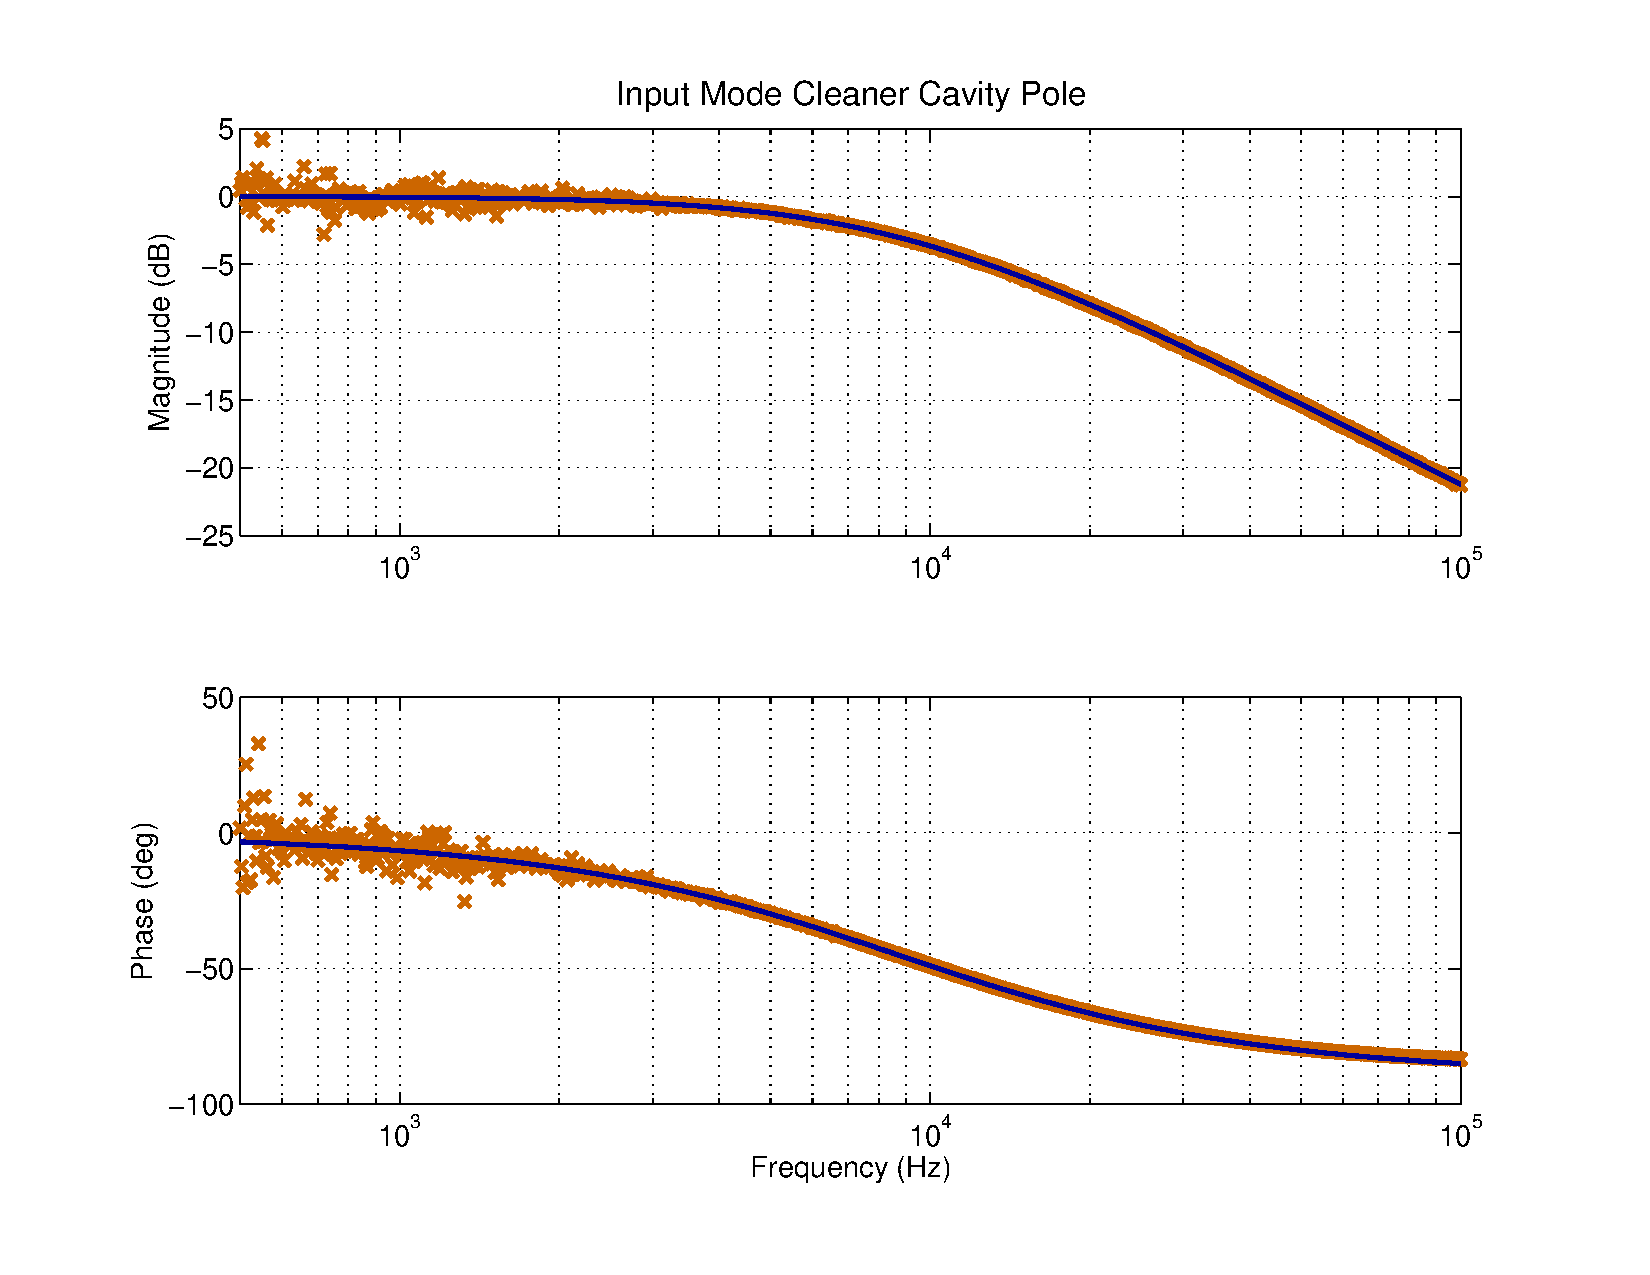
\includegraphics[width = 0.7\textwidth, trim = 2.5cm 1.5cm 2.5cm 1cm]{Cavity_Pole.pdf}
	\caption{The measured IMC cavity pole is shown together with a fit 
		to \eqref{eq:PoleApx}.  The fit has a pole frequency of 8712 Hz 
		which gives a finesse of 522.  These values are within the error 
		bars on the measured mirror reflectivies eliminating the 
		possibility of excessive losses.}
	\label{fig:cavPole}
\end{figure}

The results are shown in figure \ref{fig:cavPole} together with a fit to equation 
\eqref{eq:PoleApx}.  The results give a cavity pole of 8712 Hz which is equivalent 
to a finesse of 522.  
These numbers are exactly what was expected within the error bars of the measured 
reflectivity of the mirrors.  

%--------------------------------------------------------------------------------------------------
\subsection{Noise Budget}

%--------------------------------------------------------------------------------------------------
\subsection{Absorption Measurements}
The absorption in the input mode cleaner can be measured independently of the losses 
by tracking thermally sensitive properties of the mirrors.  
In this case we tracked two different thermally sensitive properties; 
the shift in the local radius of curvature of the optic 
and the shift in the frequency of the fundamental mechanical eigenmode of the mirror.  

The shift in the local radius of curvature of the optic was tracked by 
tracking the higher order mode spacing as a function of power.  
The spacing of the different higher order modes is dependent on the q 
parameter of the cavity which is itself dependent on the local radius of 
curvature of the mirrors.  
The Winkler et. al.\cite{Winkler1991} approximation for the local radius of 
curvature change is
\begin{equation}
	\frac{1}{\delta R}=\delta p=\frac{\alpha}{2\pi\omega^2\kappa}P_a,
\end{equation}
where $\alpha$ is the coefficient of thermal expansion of the mirror,  
$\kappa$ is the thermal conductivity, $\omega$ is the beam size, and
$P_a$ is the power absorbed by the mirror.  
Assuming that the absorption is uniform across the mirrors and the same for 
each mirror ray matrix methods can be used to derive the Gouy phase shift 
of the cavity as a function of power.  
This Gouy phase shift can be expressed equivalently as the shift in the 
frequency location of the 10 peak.  
With these assumptions and approximations the shift in the location of the 10 
peak is given by 
\begin{equation}
	\delta f_{10}=-135.1 \frac{Hz}{ppm\cdot W},
\end{equation}
where the units of ppm is per mirror rather than total.






%--------------------------------------------------------------------------------------------------
\subsection{Thermal Lensing}


\begin{thebibliography}{9}
	\bibitem{drawcite}
		Uses the vector components library developed by Alexander Franzen; available at http://www.gwoptics.org/ComponentLibrary/
	\bibitem{EricBlack}
		Eric Black's PDH paper.
	\bibitem{DreverHall}
		The Drever hall paper on the PDH technique.		
	\bibitem{Winkler1991}
		Winkler, W., K. Danzmann, A. Rudiger, and R. Schilling. Heating by Optical Absorption and 
		the Performance of Interferometric Gravitational-Wave Detectors." Phys. Rev. A 44 117022-7036. 1 December, 1991.
\end{thebibliography}		

\end{document}

%\include{chapter3a}
%\include{chapter4}
%\include{chapter5}
%\include{chapter6}

%------------------------------------------%

% Make List of References (BibTeX implemented using the Natbib package)
% un-comment your preferred bibliography style and replace the
% bibliography file "sample" with the name of your .bib file
% REMEMBER!!! If you want un-numbered references comment the Natbib package with
% The numbered options in the packages.tex file and un-comment the package with the authoryear option
% See the included pdfs of the various styles to see the differences.
% The citation style differences are from the \citet{key} and \citep{key} commands
% More options are available; see the Natbib documentation for details


\bibliography{ioPaperBib}
% You can have more than one library of references

%------------------------------------------%

\end{document}

%-------------------------------------------------------------------------------------------------------%
